\documentclass[12pt]{article}
\usepackage{graphicx}
\usepackage {color}
\usepackage{pdfpages}
\usepackage{float}
\usepackage{changebar}
\usepackage{enumitem,amssymb}
\renewcommand{\familydefault}{\sfdefault}
\usepackage[margin=1.2in]{geometry}
\usepackage{graphicx}
\usepackage{wrapfig}
\usepackage[super]{cite}
\usepackage{subcaption}
\usepackage[table]{xcolor}
\usepackage{amsmath}
\usepackage[sort, numbers]{natbib}
\usepackage{matlab-prettifier}
%%%%%%%%%%%%Defining the margins %%%%%%%%%%%%%%%%%%%%%
\textheight 9.in
\textwidth 6.5in
\topmargin -.5in
\oddsidemargin 0in
\setlength{\parskip}{\smallskipamount}

%%%%%%%%%%%%%%Specific Commands %%%%%%%%%%%%%%%%%%
\newcommand{\eg}{{\em e.g.,}}
\newcommand{\ie}{{\em i.e.,}}
\newcommand{\etc}{{\em etc.,}}
\newcommand{\etal}{{\em et al.}}
\newcommand{\degrees}{{$^{\circ}$}}
\newcommand{\micro}{{$\mu$}}


%%%%%%%%%%%%%%%%%%%%%%%%%%%% Setting to control figure placement
% These determine the rules used to place floating objects like figures 
% They are only guides, but read the manual to see the effect of each.
\renewcommand{\topfraction}{.9}
\renewcommand{\bottomfraction}{.9}
\renewcommand{\textfraction}{.1}
\renewcommand{\familydefault}{\sfdefault} %setting the san serif font

%%%%%%%%%%%%%%%%%%%%%%%% Line spacing
% Use the following command for ``double'' spacing
%\setlength{\baselineskip}{1.2\baselineskip}
% and this one for an acceptable NIH spacing of 6lpi based on 11pt
%\setlength{\baselineskip}{.9\baselineskip}
% The baselineskip does not appear to work when we include a maketitle
% command in the main file.  Something there must set the line spacing
% If we use this next command, then things seem to work.
\renewcommand{\baselinestretch}{.9}

\setcounter{secnumdepth}{0} %make no numbers but have a table of contents


\begin{document}

\title{HW 1, Propagation}
\author{Jake Bergquist, u6010393}
\maketitle

\section{1: }
In Figure~\ref{Fig:Vm} we see the resulting membrane voltage as described by Eq~\ref{eq1}, normalized to be within $\pm$1. This function only describes the upstroke of the action potential, and in this case we can use this to understand that the direction of propagation is from right to left in Figure~\ref{Fig:Vm}. 

\begin{equation}
V_m = 50*tanh(x)
\label{eq1}
\end{equation}
\begin{figure}[H]
	
	\centering
	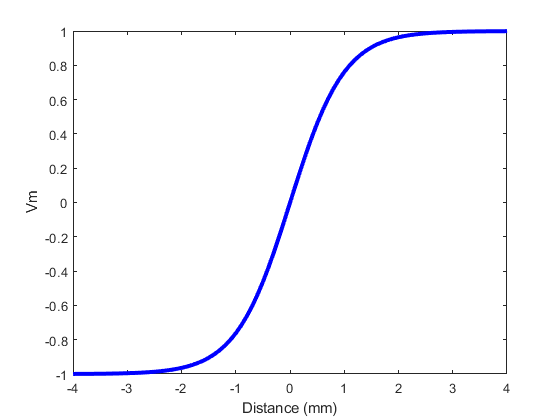
\includegraphics[width=.95\textwidth]{Figures/vm.png}
	
	\caption{Membrane voltage as a function of space along the 1D fiber. Membrane voltage has been normalized such that the peaks are at $\pm$1.}
	\label{Fig:Vm}
\end{figure}



\section{2: }
In Figure~\ref{Fig:Ii} we see the resulting intracellular current, $I_i$ as described by Eq~\ref{eq2}, normalized to be within $\pm 1$. For this lab I chose $r_e = r_i = 1$ and $I = 0$ as there is no stimulus. At the peak current the flow is the same direction of the activation, as denoted by the negative sign of the extracellular current.

\begin{equation}
I_i = \frac{-1}{r_i + r_e}(\frac{dV_m}{dx} - Ir_e)
\label{eq2}
\end{equation}
\begin{figure}[H]
	
	\centering
	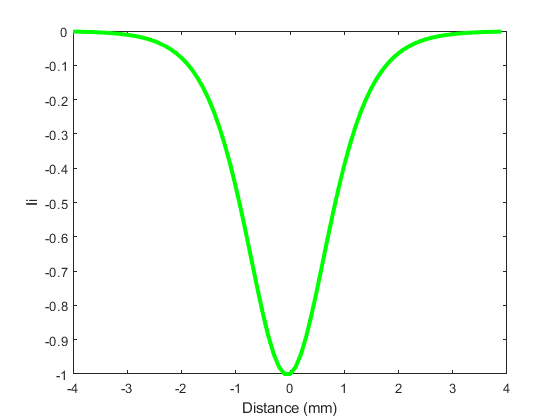
\includegraphics[width=.95\textwidth]{Figures/Ii.png}
	
	\caption{Intracellular current as a function of space along the 1D fiber. Current has been normalized such that the peak is -1.}
	\label{Fig:Ii}
\end{figure}
\section{3: }
In Figure~\ref{Fig:Ie} we see the resulting extracellular current, $I_e$ as described by Eq~\ref{eq3}, normalized to be within $\pm 1$. At the peak current the flow is the opposite direction of the activation, as denoted by the positive sign of the extracellular current.

\begin{figure}[H]
	
	\centering
	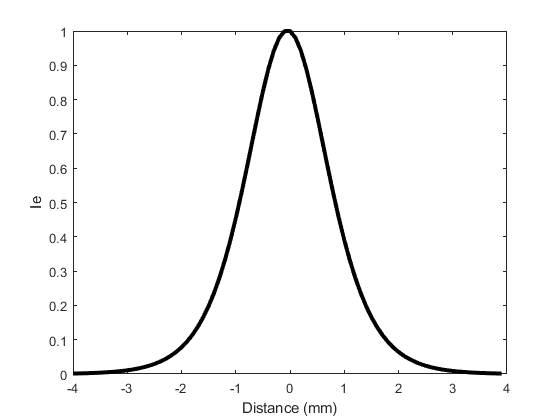
\includegraphics[width=.95\textwidth]{Figures/Ie.png}
	
	\caption{Intracellular current as a function of space along the 1D fiber. Current has been normalized such that the peak is 1.}
	\label{Fig:Ie}
\end{figure}

\begin{equation}
I_e = \frac{\frac{dV_m}{dx} + I_ir_i}{r_e}
\label{eq3}
\end{equation}

\section{4: }
In Figure~\ref{Fig:Im} we see the resulting extracellular current, $I_m$ as described by Eq~\ref{eq4}, normalized to be within $\pm 1$. At the positive peak of current we see that this aligns with the region at the wavefront of the upstroke, indicating positive current flow into the cell (sodium inflow at the wavefront as the activation spreads) while the negative peak of the membrane current corresponds to region of the wavefront that has just passed. The positive peak indicates the direction of propagation  relative to the negative peak such that propagation flows in the direction dictated as negative peak towards positive peak.
\begin{figure}[H]
	
	\centering
	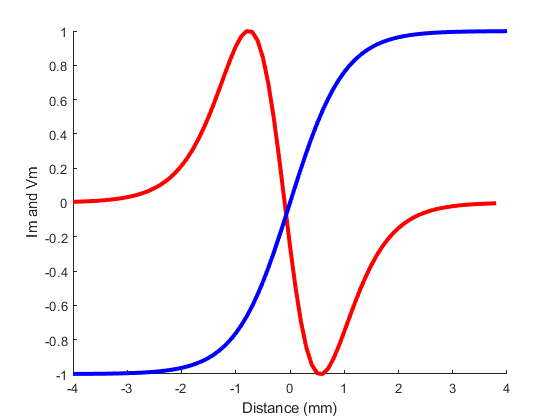
\includegraphics[width=.95\textwidth]{Figures/Im.png}
	
	\caption{Membrane current (Red) as a function of space as well as membrane voltage (blue) along the 1D fiber. Current has been normalized such that the peaks are $\pm$1. Membrane voltage has been normalized such that the peaks are $\pm$1}
	\label{Fig:Im}
\end{figure}
\begin{equation}
I_m = \frac{1}{r_i + r_e}(\frac{d^2V_m}{dx^2} - Ir_e)
\label{eq4}
\end{equation}
\section{5: }
We can solve this problem using the relationship shown in Eq~\ref{eq5}, where $S_R$ is the rheobase strength, $\tau$ is the membrane time constant, $t$ is the stimulus time we desire to use, and $S(t)$ is the strength needed to elicit an action potential given the stimulus time $t$. We can validate this by plotting the associated strength duration curve (Figure~\ref{Fig:strdur}) and see that the observed rheobase matches the $10 \mu A/cm^2$ value perscribed, and that the experimentally observed strengths and durations fall on this curve. We can now compute the required strength when using a 0.2 ms stimulus, which comes out to be $125.1 \mu A/cm^2$. This is done by evaluating Eq~\ref{eq5} using $t = 0.2ms$.

\begin{equation}
S(t) = \frac{S_R}{1-e^\frac{t}{\tau}}
\label{eq5}
\end{equation}

\begin{figure}[H]
	
	\centering
	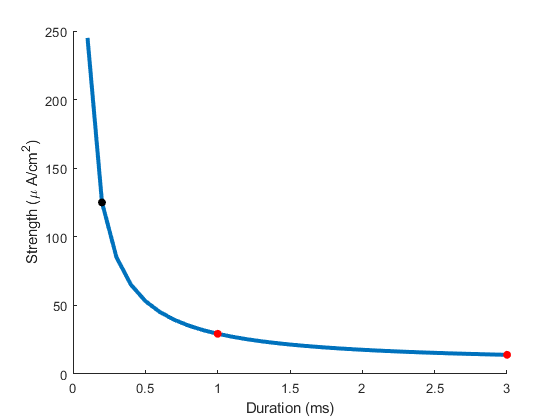
\includegraphics[width=.95\textwidth]{Figures/StrDur.png}
	
	\caption{Strength Duration curve using Eq~\ref{eq5} with $\tau = 2.4 ms$, $S_R = 10 \mu A/cm^2$. Measured points shown in red, desired measurement location shown in black.}
	\label{Fig:strdur}
\end{figure}

\section{Appendix}
All MATLAB code used to generate the figures and calculations presented in this assignment is shown below.

\begin{lstlisting}[style=Matlab-editor]

%1)
clear;close all
re = 1;
ri = 1;
x = [-4:.1:4];
vMx = 50*tanh(x);
dvMx = diff(vMx);
ddvMx = diff(dvMx);
I = 0;%No stimulation
Ii = (-1/(ri+re))*(dvMx-I*re);
Im = (1/(ri+re))*(ddvMx-I*re);
Ie = (dvMx+Ii.*ri)./re;
figure(1);
plot(x,vMx./50,'b','linewidth',3);
xlabel('Distance (mm)');
ylabel('Vm');

figure(2);
plot(x(1:end-1),Ii./(max(abs(Ii))),'g','linewidth',3)
xlabel('Distance (mm)');
ylabel('Ii');

figure(3);clf();
hold on;
plot(x(1:end-2),Im./(max(abs(Im))),'r','linewidth',3)
plot(x,vMx./50,'b','linewidth',3)
xlabel('Distance (mm)');
ylabel('Im and Vm');

figure(4);plot(x(1:end-1),Ie./(max(abs(Ie))),'k','linewidth',3)
xlabel('Distance (mm)');
ylabel('Ie');

%
%2)
rheobase = 10;%uA/cm2
durations = [1,3];
strengths = [29.346,14.015];
tc = 2.4;

t = [.1:.1:3];
Str = rheobase./(1-exp(-t/tc));
StrReq = rheobase./(1-exp(-0.2/tc));
figure(5);
hold on;
plot(t,Str,'linewidth',3)
scatter(durations,strengths,'ro','filled')
scatter(0.2,StrReq,'ko','filled');
xlabel('Duration (ms)');
ylabel('Strength (\mu A/cm^2)')





\end{lstlisting}

\end{document}








